\begin{figure}
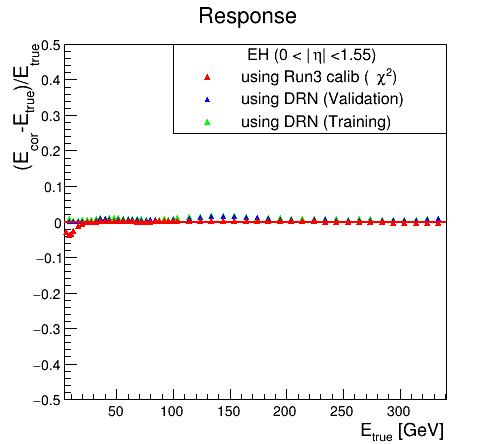
\includegraphics[width=0.495\textwidth]{./plots_pdf/HCAL_plots/Trained_target_ratioflip_0_500_10/pdf/EH_barrel/barrel_corrEtaBarrelEcalHcal.png}
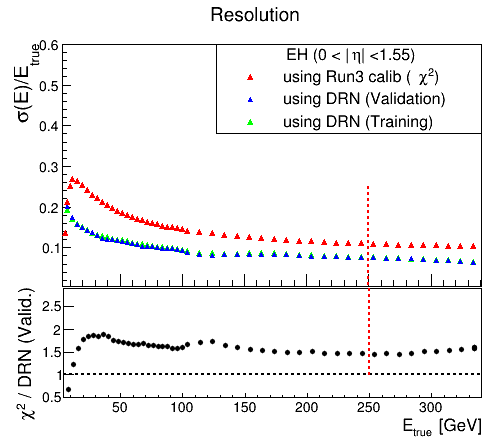
\includegraphics[width=0.495\textwidth]{./plots_pdf/HCAL_plots/Trained_target_ratioflip_0_500_10/pdf/EH_barrel/barrel_corrEtaBarrelEcalHcal_reso.png}

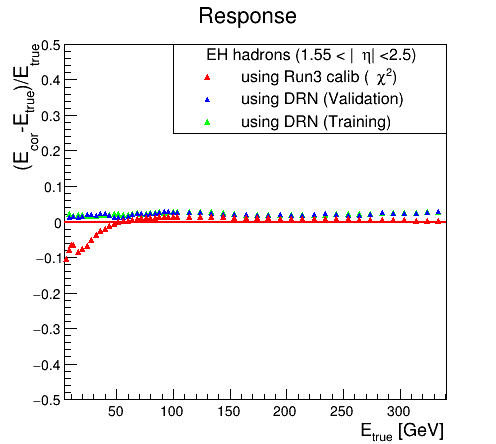
\includegraphics[width=0.495\textwidth]{./plots_pdf/HCAL_plots/Trained_target_ratioflip_0_500_10/pdf/EH_ec_in/EC_within_tracker_corrEtaEndcapEcalHcal.png}
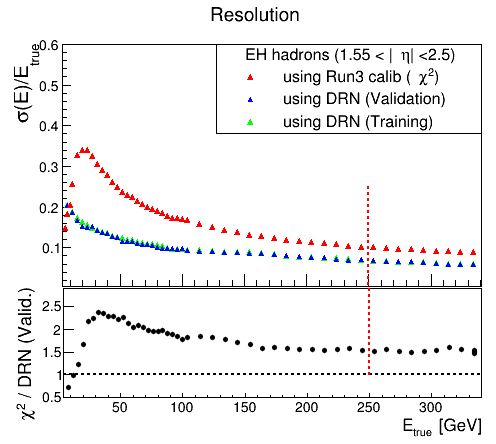
\includegraphics[width=0.495\textwidth]{./plots_pdf/HCAL_plots/Trained_target_ratioflip_0_500_10/pdf/EH_ec_in/EC_within_tracker_corrEtaEndcapEcalHcal_reso.png}

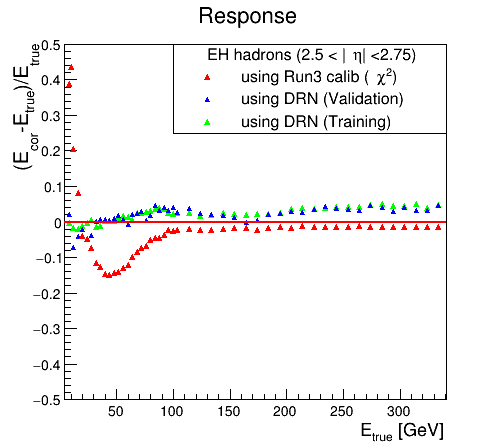
\includegraphics[width=0.495\textwidth]{./plots_pdf/HCAL_plots/Trained_target_ratioflip_0_500_10/pdf/EH_ec_out/EC_outside_tracker_corrEtaEndcapEcalHcal.png}
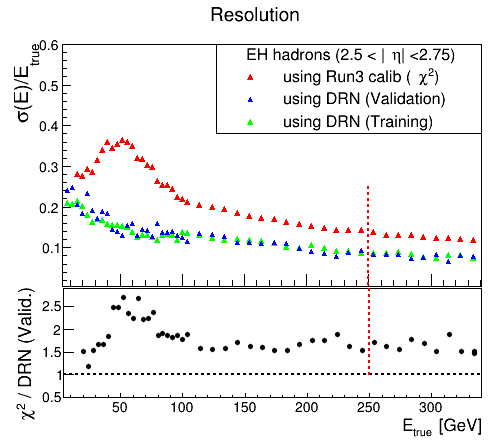
\includegraphics[width=0.495\textwidth]{./plots_pdf/HCAL_plots/Trained_target_ratioflip_0_500_10/pdf/EH_ec_out/EC_outside_tracker_corrEtaEndcapEcalHcal_reso.png}

\caption[ Response (resolution) vs \pt of the PF EH-hadron cluster - traget log(ratioflip)]{Mean response (resolution) defined by calibrated PF EH-hadron clusters using $\chi^{2}$ method (red), DRN modle derivedfrom training samples (green), DRN modle validated on testing samples (blue). (top) barrel, (middle) endcap within tracker, (bottom) endcap outside the tracker. DRN training target is log(ratioflip)}
\label{fig:EH_logratioflip}
\end{figure}
